\documentclass[10pt]{./IEEEtran}

% Some very useful LaTeX packages include:
% (uncomment the ones you want to load)


% *** MISC UTILITY PACKAGES ***
%
%\usepackage{ifpdf}
% Heiko Oberdiek's ifpdf.sty is very useful if you need conditional
% compilation based on whether the output is pdf or dvi.
% usage:
% \ifpdf
%   % pdf code
% \else
%   % dvi code
% \fi
% The latest version of ifpdf.sty can be obtained from:
% http://www.ctan.org/tex-archive/macros/latex/contrib/oberdiek/
% Also, note that IEEEtran.cls V1.7 and later provides a builtin
% \ifCLASSINFOpdf conditional that works the same way.
% When switching from latex to pdflatex and vice-versa, the compiler may
% have to be run twice to clear warning/error messages.






% *** CITATION PACKAGES ***
%
\usepackage{cite}
% cite.sty was written by Donald Arseneau
% V1.6 and later of IEEEtran pre-defines the format of the cite.sty package
% \cite{} output to follow that of IEEE. Loading the cite package will
% result in citation numbers being automatically sorted and properly
% "compressed/ranged". e.g., [1], [9], [2], [7], [5], [6] without using
% cite.sty will become [1], [2], [5]--[7], [9] using cite.sty. cite.sty's
% \cite will automatically add leading space, if needed. Use cite.sty's
% noadjust option (cite.sty V3.8 and later) if you want to turn this off.
% cite.sty is already installed on most LaTeX systems. Be sure and use
% version 4.0 (2003-05-27) and later if using hyperref.sty. cite.sty does
% not currently provide for hyperlinked citations.
% The latest version can be obtained at:
% http://www.ctan.org/tex-archive/macros/latex/contrib/cite/
% The documentation is contained in the cite.sty file itself.






% *** GRAPHICS RELATED PACKAGES ***
%
\ifCLASSINFOpdf
  \usepackage[pdftex]{graphicx}
  % declare the path(s) where your graphic files are
  % \graphicspath{{../pdf/}{../jpeg/}}
  % and their extensions so you won't have to specify these with
  % every instance of \includegraphics
  % \DeclareGraphicsExtensions{.pdf,.jpeg,.png}
\else
  % or other class option (dvipsone, dvipdf, if not using dvips). graphicx
  % will default to the driver specified in the system graphics.cfg if no
  % driver is specified.
  % \usepackage[dvips]{graphicx}
  % declare the path(s) where your graphic files are
  % \graphicspath{{../eps/}}
  % and their extensions so you won't have to specify these with
  % every instance of \includegraphics
  % \DeclareGraphicsExtensions{.eps}
\fi
% graphicx was written by David Carlisle and Sebastian Rahtz. It is
% required if you want graphics, photos, etc. graphicx.sty is already
% installed on most LaTeX systems. The latest version and documentation can
% be obtained at: 
% http://www.ctan.org/tex-archive/macros/latex/required/graphics/
% Another good source of documentation is "Using Imported Graphics in
% LaTeX2e" by Keith Reckdahl which can be found as epslatex.ps or
% epslatex.pdf at: http://www.ctan.org/tex-archive/info/
%
% latex, and pdflatex in dvi mode, support graphics in encapsulated
% postscript (.eps) format. pdflatex in pdf mode supports graphics
% in .pdf, .jpeg, .png and .mps (metapost) formats. Users should ensure
% that all non-photo figures use a vector format (.eps, .pdf, .mps) and
% not a bitmapped formats (.jpeg, .png). IEEE frowns on bitmapped formats
% which can result in "jaggedy"/blurry rendering of lines and letters as
% well as large increases in file sizes.
%
% You can find documentation about the pdfTeX application at:
% http://www.tug.org/applications/pdftex





% *** MATH PACKAGES ***
%
%\usepackage[cmex10]{amsmath}
% A popular package from the American Mathematical Society that provides
% many useful and powerful commands for dealing with mathematics. If using
% it, be sure to load this package with the cmex10 option to ensure that
% only type 1 fonts will utilized at all point sizes. Without this option,
% it is possible that some math symbols, particularly those within
% footnotes, will be rendered in bitmap form which will result in a
% document that can not be IEEE Xplore compliant!
%
% Also, note that the amsmath package sets \interdisplaylinepenalty to 10000
% thus preventing page breaks from occurring within multiline equations. Use:
%\interdisplaylinepenalty=2500
% after loading amsmath to restore such page breaks as IEEEtran.cls normally
% does. amsmath.sty is already installed on most LaTeX systems. The latest
% version and documentation can be obtained at:
% http://www.ctan.org/tex-archive/macros/latex/required/amslatex/math/
\usepackage{mathrsfs}



% *** SPECIALIZED LIST PACKAGES ***
%
%\usepackage{algorithmic}
% algorithmic.sty was written by Peter Williams and Rogerio Brito.
% This package provides an algorithmic environment fo describing algorithms.
% You can use the algorithmic environment in-text or within a figure
% environment to provide for a floating algorithm. Do NOT use the algorithm
% floating environment provided by algorithm.sty (by the same authors) or
% algorithm2e.sty (by Christophe Fiorio) as IEEE does not use dedicated
% algorithm float types and packages that provide these will not provide
% correct IEEE style captions. The latest version and documentation of
% algorithmic.sty can be obtained at:
% http://www.ctan.org/tex-archive/macros/latex/contrib/algorithms/
% There is also a support site at:
% http://algorithms.berlios.de/index.html
% Also of interest may be the (relatively newer and more customizable)
% algorithmicx.sty package by Szasz Janos:
% http://www.ctan.org/tex-archive/macros/latex/contrib/algorithmicx/




% *** ALIGNMENT PACKAGES ***
%
%\usepackage{array}
% Frank Mittelbach's and David Carlisle's array.sty patches and improves
% the standard LaTeX2e array and tabular environments to provide better
% appearance and additional user controls. As the default LaTeX2e table
% generation code is lacking to the point of almost being broken with
% respect to the quality of the end results, all users are strongly
% advised to use an enhanced (at the very least that provided by array.sty)
% set of table tools. array.sty is already installed on most systems. The
% latest version and documentation can be obtained at:
% http://www.ctan.org/tex-archive/macros/latex/required/tools/


%\usepackage{mdwmath}
%\usepackage{mdwtab}
% Also highly recommended is Mark Wooding's extremely powerful MDW tools,
% especially mdwmath.sty and mdwtab.sty which are used to format equations
% and tables, respectively. The MDWtools set is already installed on most
% LaTeX systems. The lastest version and documentation is available at:
% http://www.ctan.org/tex-archive/macros/latex/contrib/mdwtools/


% IEEEtran contains the IEEEeqnarray family of commands that can be used to
% generate multiline equations as well as matrices, tables, etc., of high
% quality.


%\usepackage{eqparbox}
% Also of notable interest is Scott Pakin's eqparbox package for creating
% (automatically sized) equal width boxes - aka "natural width parboxes".
% Available at:
% http://www.ctan.org/tex-archive/macros/latex/contrib/eqparbox/





% *** SUBFIGURE PACKAGES ***
%\usepackage[tight,footnotesize]{subfigure}
% subfigure.sty was written by Steven Douglas Cochran. This package makes it
% easy to put subfigures in your figures. e.g., "Figure 1a and 1b". For IEEE
% work, it is a good idea to load it with the tight package option to reduce
% the amount of white space around the subfigures. subfigure.sty is already
% installed on most LaTeX systems. The latest version and documentation can
% be obtained at:
% http://www.ctan.org/tex-archive/obsolete/macros/latex/contrib/subfigure/
% subfigure.sty has been superceeded by subfig.sty.



%\usepackage[caption=false]{caption}
%\usepackage[font=footnotesize]{subfig}
% subfig.sty, also written by Steven Douglas Cochran, is the modern
% replacement for subfigure.sty. However, subfig.sty requires and
% automatically loads Axel Sommerfeldt's caption.sty which will override
% IEEEtran.cls handling of captions and this will result in nonIEEE style
% figure/table captions. To prevent this problem, be sure and preload
% caption.sty with its "caption=false" package option. This is will preserve
% IEEEtran.cls handing of captions. Version 1.3 (2005/06/28) and later 
% (recommended due to many improvements over 1.2) of subfig.sty supports
% the caption=false option directly:
%\usepackage[caption=false,font=footnotesize]{subfig}
%
% The latest version and documentation can be obtained at:
% http://www.ctan.org/tex-archive/macros/latex/contrib/subfig/
% The latest version and documentation of caption.sty can be obtained at:
% http://www.ctan.org/tex-archive/macros/latex/contrib/caption/




% *** FLOAT PACKAGES ***
%
%\usepackage{fixltx2e}
% fixltx2e, the successor to the earlier fix2col.sty, was written by
% Frank Mittelbach and David Carlisle. This package corrects a few problems
% in the LaTeX2e kernel, the most notable of which is that in current
% LaTeX2e releases, the ordering of single and double column floats is not
% guaranteed to be preserved. Thus, an unpatched LaTeX2e can allow a
% single column figure to be placed prior to an earlier double column
% figure. The latest version and documentation can be found at:
% http://www.ctan.org/tex-archive/macros/latex/base/



%\usepackage{stfloats}
% stfloats.sty was written by Sigitas Tolusis. This package gives LaTeX2e
% the ability to do double column floats at the bottom of the page as well
% as the top. (e.g., "\begin{figure*}[!b]" is not normally possible in
% LaTeX2e). It also provides a command:
%\fnbelowfloat
% to enable the placement of footnotes below bottom floats (the standard
% LaTeX2e kernel puts them above bottom floats). This is an invasive package
% which rewrites many portions of the LaTeX2e float routines. It may not work
% with other packages that modify the LaTeX2e float routines. The latest
% version and documentation can be obtained at:
% http://www.ctan.org/tex-archive/macros/latex/contrib/sttools/
% Documentation is contained in the stfloats.sty comments as well as in the
% presfull.pdf file. Do not use the stfloats baselinefloat ability as IEEE
% does not allow \baselineskip to stretch. Authors submitting work to the
% IEEE should note that IEEE rarely uses double column equations and
% that authors should try to avoid such use. Do not be tempted to use the
% cuted.sty or midfloat.sty packages (also by Sigitas Tolusis) as IEEE does
% not format its papers in such ways.





% *** PDF, URL AND HYPERLINK PACKAGES ***
%
%\usepackage{url}
% url.sty was written by Donald Arseneau. It provides better support for
% handling and breaking URLs. url.sty is already installed on most LaTeX
% systems. The latest version can be obtained at:
% http://www.ctan.org/tex-archive/macros/latex/contrib/misc/
% Read the url.sty source comments for usage information. Basically,
% \url{my_url_here}.





% *** Do not adjust lengths that control margins, column widths, etc. ***
% *** Do not use packages that alter fonts (such as pslatex).         ***
% There should be no need to do such things with IEEEtran.cls V1.6 and later.
% (Unless specifically asked to do so by the journal or conference you plan
% to submit to, of course. )


% correct bad hyphenation here
\hyphenation{op-tical net-works semi-conduc-tor}


\begin{document}

\title{Federation Among Remote Military Data Stores In Austere Environments}

\author{\IEEEauthorblockN{Steven Mazza}\\
\IEEEauthorblockA{School of Systems Engineering\\
Naval Postgraduate School\\
Monterey, CA 93943\\
Email: spmazza@nps.edu}}


% make the title area
\maketitle


\begin{abstract}
%\boldmath
Transportable computing and some degree of network connectivity have been a necessary component of US military operations at least since the advent of the personal computer in the 1980s.  Subsequent ubiquity of laptop computers and, more recently, hand held devices such as the smart phone have exacerbated the situation by allowing the need for data and the locus of computing power to be increasingly distributed and fragmented.  Through model design and discussion we address some aspects of one potential solution to this fragmentation through federation of data stores.  In particular, we show that we can guarantee eventual consistency of data, even in austere environments.  Furtherore, we show that this state can be achieved in time proportional to $O(K log(n))$ where $n$ is the number of nodes in the network.

%TODO: fix the metrics.
\end{abstract}


\IEEEpeerreviewmaketitle


\section{Introduction}
\label{sec:introduction}
% no \IEEEPARstart
Transportable computing and some degree of network connectivity have been a necessary component of US military operations at least since the advent of the personal computer in the 1980s.  Subsequent ubiquity of laptop computers and, more recently, hand held devices such as the smart phone have exacerbated the situation by allowing the need for data and the locus of computing power to be increasingly distributed and fragmented.  

Consequently, there exists a significant and growing problem related to the decentralization of computing in the United States military.  Due to the increasing distribution of computing power and data storage, there is now an acknowledged need to implement some form of federation\cite{Takai:2012} in order to maintain data concurrency.  This is especially true in theaters of operation that are characterized as austere environments and for which communications are assumed to be disconnected, intermittent, or limited (DIL), and where connections to a centralized data store are impractical or impossible\cite{Sonnenberg:2009}.

The paper is structured as follows.  We begin in Section \ref{sec:probspace} by introducing the problem space, which includes a discussion of the motivation for this work along with the questions we address.  Section \ref{sec:doe} sets up the design of experiments that we use to address the questions introduced in Section \ref{sec:probspace}.  Next we dive into a discussion of the model design in Section \ref{sec:model}.  We discuss the model development and constraints including bandwidth and connectivity, edge construction, and graph topology.  Disaster recovery is briefly related to our study in Section \ref{sec:dr}, and we wrap up with related work in Section \ref{sec:related} and finally a conclusion in Section \ref{sec:conclusion}.


\section{Problem Space}
\label{sec:probspace}
United States involvement in military operations over the past fifteen years has been in operationally challenging environments.  Lack of existing infrastructure to provide necessary operational support has been a primary challenge to sustaining long-term presence necessary to achieve our national security goals.  We focus on the challenges associated with fighting in an asymmetrical conflict while operating in an environment in which the transmission of electronic data is challenging at best.

\subsection{Motivation}
Maintaining some data consistency in support of military operations is an important component to ensuring that everyone is working from the same basis of understanding in carrying out the Commander's intent.\footnote{Commander's intent in the military context is the broad context under which both direction is given by 06 officers and specific actions are taken by MAJ and SGT warfighters.}  If a given unit in formation is working off of a differential of understanding due either to stale or missing data, that unit runs the risk of inadvertently placing others in harm's way.

Data can be relatively immutable and persist for long periods of time, as with terrain maps which tend to change on a geologic scale.  On the other hand much of the important data is highly volatile and often takes the form of overlays on the maps.  Data such as current friendly force and enemy positions, locations of supply and weapons cache, and route planning characterize this type of data.  Intelligence data, recent significant events, and UAS feeds all have a relatively short shelf life and tend to get updated frequently.

This type of data is typical of that which is both produced and consumed by many programs of record (PoRs).\footnote{Examples in the US Army include Command Post of the Future (CPoF) and Joint Battle Command Platform (JBC-P)}  Programs of record refer to systems that are fielded by Program Management organizations in the Army and comprise the tools with which warfighters accomplish their jobs.  In the absence of a unified mechanism and in an effort to ensure the best information is delivered to the warfighter at any point, each of these PoRs attempts to address the problems of federation, individually.

This presents a problem for the military for several reasons.  On the surface, stove-piped solutions present an ongoing barrier to interoperability and compatibility.  But on a more fundamental level, there exists a commonality for the need to have access to federation as a service.  In this way the military can proactively protect and manage bandwidth as an organizational resource.  We want to view bandwidth, for example, as a resource and treat it similarly to ammunition and food.


\subsection{Questions}
Here is what we intend to address.  We would like to know if we can guarantee the eventual consistency of data, if even statistically.  Furthermore, we would like to know in what sort of time can we expect to achieve data consistency. For the investigation of these concerns we will address time as a function of algorithmic complexity\footnote{We express complexity in big O notation.}, although that could easily be extrapolated to an estimate of elapsed time.


\section{Design of Experiments}
\label{sec:doe}
We begin by constructing an acyclic undirected graph as described in Section \ref{sec:model} with $k$ nodes.  We assign some $\rho$ data elements to each node, and assume unlimited capacity.  Storage is not expensive, and the cost per unit storage is dropping in excess of that predicted by Moore's Law.  Consequently, any accounting for capacity as a significant factor will be rapidly made obsolete by the market.  Furthermore, as connectivity increases, we may begin to naturally favor solutions such as a dynamic distributed federated database (DDFD) which allow queries to be distributed across the network\cite{Bent2009}.

We first measure the time steps, $t$, required to synchronize all $n$ nodes of the network with $\rho$ elements of data, and show that this operation completes in polynomial time.  Next we re-establish our initial conditions and run our experiment again with the introduction of randomly assigned edges, creating temporary cycles in the graph.  These edges are assigned as follows.

We select two non-adjacent nodes, $\mathscr{N}_{i}$ and $\mathscr{N}_{j}$, of the graph at random, with probability proportional to their connectivity within their respective immediate neighbors, $p(\mathscr{N}_{i})$ and $p(\mathscr{N}_{j})$, which we can refer to as $p_{i}$ and $p_{j}$ for convenience.  We allow the newly created edge to persist for one time step during which both nodes can perform a full exchange of data.  Note that it is possible, given sufficiently low probability of overall connectivity, that no new edge will be created on any given time step, $\tau_{t}$.  At most, however, one edge will be constructed.


\section{Model Design}
\label{sec:model}
We have an interesting situation in that the physical organization of the network is highly structured, as prescribed by military doctrine, which favors a top-down, hierarchical task organization with a relatively fixed number of nodes at each echelon.  We generalize this as a tree structure in the classical sense, having no closed loops.  We then augment this structure by introducing some loops that connect nodes both laterally and across echelons to represent various opportunities for data delivery and synchronization scenarios not uncommon to actual operational threads.

\subsection{Bandwidth and Connectivity}

Where this graph structure becomes particularly interesting is in the implementation of the edges.  Due to limited resources in most all theaters of operation\footnote{At the time of the writing of this paper, recent theaters of operation included Iran, Iraq, and Afghanistan.} we model the probability of connectivity and bandwidth as an edge weight that tends to follow an inverse power formula proportional to the distance of any node, $\mathscr{N}_{k}$, to the root node, $\mathscr{N}_{0}$.  Figure \ref{fig:probcon} shows a range of representative probabilities of connectivity that might suit a model given a variety of working environmental conditions.  We develop a plot of the probability by echelon and vary the overall likelihood by altering $n$ to suit measurable conditions.

\begin{figure}[h!]
  \centering
    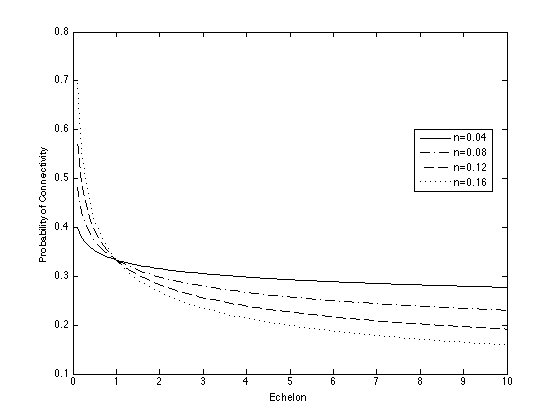
\includegraphics[width=0.5\textwidth]{images/probcon}
  \caption{Representative probabilities of connectivity by echelon, given various conditions.}
  \label{fig:probcon}
\end{figure}

We allow creation of the graph model dynamically by using an inverse power formula to approximate both bandwidth and the probability of connectivity within the constraints of our graph model.  We can see this illustrated in Figure \ref{fig:bandwidth}.  We assume distance, $d$, as the graph distance between any two given nodes, $\mathscr{N}_i$ and $\mathscr{N}_j$ such that $d(\mathscr{N}_{i}, \mathscr{N}_{j})$ is the geodesic distance with $0<d\leq \epsilon(v)$, where $\epsilon(v)$ is the graph diameter.  We construct the graph following this basic model but adjust the value, $K$, to allow a correction for the particular constraints of any specific environment.

\begin{figure}[h!]
  \centering
    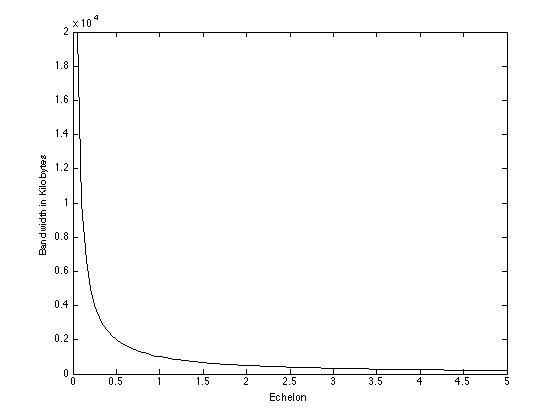
\includegraphics[width=0.5\textwidth]{images/bandwidth}
  \caption{Example representation of bandwidth by echelon.}
  \label{fig:bandwidth}
\end{figure}

\subsection{Undirected Graph}
While the traditional flow of information in a military hierarchy follows a top-down model, we implement an undirected graph.  We feel this is in keeping with the stated specific desire that each soldier become a sensor on the network\cite{Patton:2003}.  A direct result of this is that information will naturally flow naturally both up and down the traditional chain of command.  An unintended consequence is that, due largely to task re-organization, general officer and staff mobility, and transient network connections, it may also flow laterally within a structural organization and even across formations.  We will further see how this occasional lateral flow of information facilitates our desired end state of achieving consistency of data across the network by creating temporary ad hoc small-world networks within the hierarchical military structure.

\subsection{Shortcuts}
We intentionally allow the occasional introduction of shortcuts on our graph.  These shortcuts model the transit of information over non-traditional routes within the network.  This is illustrated in Figure \ref{fig:network}.  Shortcuts are an important part of this network model in that they intermittently create small-world type situations\cite{Vahdat:2000} within an otherwise hierarchical, acyclical network model.  These shortcuts come in two general types that have similar effect but which arise from different circumstances.

\subsubsection{Lateral Movement of Data} 
Data at rest on computing devices\footnote{While these are traditionally ruggedized racked computers, increasingly they will be tablets, smart phones, and other end user devices (EUDs).} in transit between Companies or Battalions is an example of how a situation can arise.  When this results in the opportunistic exchange and synchronization of data between nodes that are otherwise separated by much larger geodesic distances,  it constitutes an instance of an unintended consequence of an increasingly distributed and mobile computing environment.

\begin{figure}[h!]
  \centering
    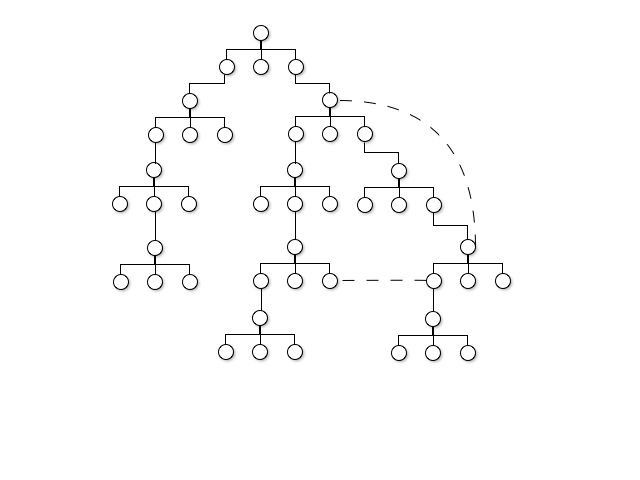
\includegraphics[width=0.5\textwidth]{images/network}
  \caption{Representative lateral and hierarchical cycles.}
  \label{fig:network}
\end{figure}

\subsubsection{Hierarchical Movement of Data}
The establishment of temporary connectivity from one echelon to another, which bypasses the standard chain of command can also result in a hierarchical movement of data.  Such situation may exist if, for example, a Company Commander required a Sat-Com link to a Division asset or if that Commander (or his staff) travels to Division HQ.  In both cases we are creating network cycles in the form of temporary links that transcend the hierarchical structure of the graph and connect nodes that are otherwise separated by much larger geodesic distances.  This has a nontrivial effect\cite{Ganesh:2005} on rate at which data is disseminated across the network.


\section{Disaster Recovery}
\label{sec:dr}
An event in which a node suffers catastrophic loss of data, characterized as a disaster recovery scenario, can be evaluated with epidemic modeling.  In both cases there is a non-trivial healing function which occurs over some $t$ time steps and which is affected by the network topology\cite{Ganesh:2005}.  In the former case, the disaster recovery \emph{heals} similar to a standard S-I-R model.  The failed node is analogous to the infected state (as in a cellular automata).  As the data propagates back, the infected node transitions to a recovered state.  All nodes on the network are assumed to be susceptible.  

As with all data flow on the network, the rate of propagation of data to the failed node is determined by bandwidth and probability of connectivity, both of which have been previously defined in terms of their geodesic distance to the root node.  A complete discussion of this additional modeling is left to future work.


\section{Related Work}
\label{sec:related}
Given the rapidly evolving nature of both military conflict and technology, there are many opportunities to extend and enhance this work.  Possibilities for additional related work include the following.

Individual datum may have different levels of importance, and consequently there may be the need to address QoS issues on the network.  In the context investigated in this paper, all data are treated equally on the network and there is no attempt made to differentiate datum, sender, or recipient, although all three might be a valid basis for establishing precedence.

Especially in a military context, but in others as well, there is a need to control access to data based on different criteria.  Frequently this tames the form of access list or is managed through credentials during sign-on.  Security has been summarily ignored for the sake of this discussion, but must be implemented in a way that satisfies the needs of the organization.  In many situations this extends not only to controlling data access by individuals on the network but also controlling what data reaches the network in the first place.  In the military this is sometimes referred to as a red-black issue and much of the concern over security revolves around defending network borders.
	
Earlier, we briefly mentioned dynamic distributed federated databases (DDFDs) and suggested that there might at some future point be an opportunity to assess their fitness for use in austere conditions.  They are popular and will become a viable solution as network capacity and reliability continue to increase or where data needs are sufficiently localized and local connectivity allows.

\section{Conclusion}
\label{sec:conclusion}
The conclusion goes here.


% An example of a floating figure using the graphicx package.
% Note that \label must occur AFTER (or within) \caption.
% For figures, \caption should occur after the \includegraphics.
% Note that IEEEtran v1.7 and later has special internal code that
% is designed to preserve the operation of \label within \caption
% even when the captionsoff option is in effect. However, because
% of issues like this, it may be the safest practice to put all your
% \label just after \caption rather than within \caption{}.
%
% Reminder: the "draftcls" or "draftclsnofoot", not "draft", class
% option should be used if it is desired that the figures are to be
% displayed while in draft mode.
%
%\begin{figure}[!t]
%\centering
%\includegraphics[width=2.5in]{myfigure}
% where an .eps filename suffix will be assumed under latex, 
% and a .pdf suffix will be assumed for pdflatex; or what has been declared
% via \DeclareGraphicsExtensions.
%\caption{Simulation Results}
%\label{fig_sim}
%\end{figure}

% Note that IEEE typically puts floats only at the top, even when this
% results in a large percentage of a column being occupied by floats.


% An example of a double column floating figure using two subfigures.
% (The subfig.sty package must be loaded for this to work.)
% The subfigure \label commands are set within each subfloat command, the
% \label for the overall figure must come after \caption.
% \hfil must be used as a separator to get equal spacing.
% The subfigure.sty package works much the same way, except \subfigure is
% used instead of \subfloat.
%
%\begin{figure*}[!t]
%\centerline{\subfloat[Case I]\includegraphics[width=2.5in]{subfigcase1}%
%\label{fig_first_case}}
%\hfil
%\subfloat[Case II]{\includegraphics[width=2.5in]{subfigcase2}%
%\label{fig_second_case}}}
%\caption{Simulation results}
%\label{fig_sim}
%\end{figure*}
%
% Note that often IEEE papers with subfigures do not employ subfigure
% captions (using the optional argument to \subfloat), but instead will
% reference/describe all of them (a), (b), etc., within the main caption.


% An example of a floating table. Note that, for IEEE style tables, the 
% \caption command should come BEFORE the table. Table text will default to
% \footnotesize as IEEE normally uses this smaller font for tables.
% The \label must come after \caption as always.
%
%\begin{table}[!t]
%% increase table row spacing, adjust to taste
%\renewcommand{\arraystretch}{1.3}
% if using array.sty, it might be a good idea to tweak the value of
% \extrarowheight as needed to properly center the text within the cells
%\caption{An Example of a Table}
%\label{table_example}
%\centering
%% Some packages, such as MDW tools, offer better commands for making tables
%% than the plain LaTeX2e tabular which is used here.
%\begin{tabular}{|c||c|}
%\hline
%One & Two\\
%\hline
%Three & Four\\
%\hline
%\end{tabular}
%\end{table}


% Note that IEEE does not put floats in the very first column - or typically
% anywhere on the first page for that matter. Also, in-text middle ("here")
% positioning is not used. Most IEEE journals/conferences use top floats
% exclusively. Note that, LaTeX2e, unlike IEEE journals/conferences, places
% footnotes above bottom floats. This can be corrected via the \fnbelowfloat
% command of the stfloats package.



%The following is just a collection of citations that may (or may not) be used in this paper.  I have collected them here in order to ensure they not get misplaced.
%\cite{Hui:2011}\cite{Liu:2009}\cite{Vahdat:2000}\cite{Gross:2006}\cite{Fu:2003}\cite{Ganesh:2005}
%\cite{Bent2009}\cite{Bent:2008}\cite{Toce:2011}\cite{Sonnenberg:2009}



% conference papers do not normally have an appendix


% use section* for acknowledgement
\section*{Acknowledgment}
%
%
The authors would like to thank Dr. Timothy Chung and the Systems Engineering Department of the Naval Postgraduate School for their support, resources, and motivation.





% trigger a \newpage just before the given reference
% number - used to balance the columns on the last page
% adjust value as needed - may need to be readjusted if
% the document is modified later
%\IEEEtriggeratref{8}
% The "triggered" command can be changed if desired:
%\IEEEtriggercmd{\enlargethispage{-5in}}

% references section

% can use a bibliography generated by BibTeX as a .bbl file
% BibTeX documentation can be easily obtained at:
% http://www.ctan.org/tex-archive/biblio/bibtex/contrib/doc/
% The IEEEtran BibTeX style support page is at:
% http://www.michaelshell.org/tex/ieeetran/bibtex/
\bibliographystyle{IEEEtran}
% argument is your BibTeX string definitions and bibliography database(s)
\bibliography{../../581Thesis/bibtex/581}
%
% <OR> manually copy in the resultant .bbl file
% set second argument of \begin to the number of references
% (used to reserve space for the reference number labels box)
%\begin{thebibliography}{1}
%
%\end{thebibliography}




% that's all folks
\end{document}


